\documentclass{article}

%............Inicia Preambulo.......................
\usepackage{graphicx}
\usepackage{float}
\usepackage[utf8]{inputenc}
\usepackage[shortlabels]{enumitem}
\usepackage{textcomp}
\usepackage{multicol}
\usepackage{caption}
\usepackage{amsfonts}
\usepackage[spanish]{babel}
\usepackage[total={17.5cm, 23cm}, top=2cm, left=2cm]{geometry}
\usepackage{esvect}
\usepackage[font=footnotesize]{caption}

\spanishdecimal{.}
\parindent 0cm

%.............Fin de Preambulo........................

\begin{document}

\begin{center}
{\Large \textbf{Universidad Autónoma de Coahuila}}
\end{center}

\begin{center}
{\large Facultad de Ciencias Físico-Matemáticas}
\end{center}

%Materia
\begin{center}
{\large Metodos Numericos}
\end{center}

%Título
\begin{center}
{\large Series de Taylor}
\end{center}

%Fecha
\begin{center}
{\large 29 de Noviembre del 2019}
\end{center}

%Autor
\begin{center}
{\large José Antonio Olveda García}
\end{center}

\vspace{5mm}

\begin{multicols}{2}

\section{Objetivo}
\label{sec:Obj}
Analizar el metodo de resolucion de aproximaciones de funciones complicadas por medio del metodo de series de taylor.

\section{Introduccion}
\label{Intro}
Una serie de Taylor es una aproximación de funciones mediante una serie de potencias o suma de potencias enteras de polinomios. 

\section{Metodologia}
\label{sec:Met}
Suponga que $\mathcal{F} \epsilon$ $\mathbb{C}^{n}$, que $\mathcal{F}^{n+1}$ existe en $[a,b]$ y $x_{0} \epsilon [a,b]$. Para cada x$\epsilon [a,b]$, existe un numero $\varepsilon (x)$ entre $x_{0}$ y x tal que 
\begin{center}
$\mathcal{F}(x)= \mathcal{P}_{n}(x) + \mathcal{R}_{n}(x)$
\\
donde 
\\
$\mathcal{P}_{n}(x) = \mathcal{F}(x_{0}) + \mathcal{F}'(x_{0})(x-x_{0})+\frac{\mathcal{F}''(x_{0})}{2!}(x-x_{0})^{2}+...+ \frac{\mathcal{F}^{n}(x_{0})}{n!}(x-x_{0})^{n}$
\\
\begin{equation}
\sum_{k=0}^{n} \frac{\mathcal{F}(x_{0})}{k!}(x-x_{0})^{k}
\end{equation}
y
\begin{equation}
\mathcal{R}_{n}(x)=\frac{\mathcal{F}^(n+1)(\varepsilon (x))}{(n+1)!}(x-x_{0})^{n+1}
\end{equation}

\end{center} 
En este caso, $\mathcal{P}_{n}(x)$ es el n-esimo polinomio de Taylor para $\mathcal{f}$ respecto de $x_{0}$, y $\mathcal{R}_{n}$ se llama el \textbf{termino del residuo (o error de truncamiento)} asociada a  $\mathcal{P}_{n}(x)$. La serie infinita obtenida al tomar el limite  de $\mathcal{P}_{n}(x)$ cuando $n \longrightarrow \infty$ es la \textbf{Serie de Taylor} para $\mathcal{F}$ en torno a $x_{0}$. En el caso $x_{0}$=0, el polinomio de taylor suele llamarse \textbf{polinomio de Maclaurin}, y la serie se nombra \textbf{serie de Maclaurin}.
\\
El termino error de truncamiento se refiere al error implicito al usar una suma truncada, o finita, para aproximar la suma de una serie infinita

\section{Ejemplo del manejo de Taylor}
\label{sec:Ejemplo}
Ejemplo
\\
Determine $a$ el segundo y $b$ el tercer polinomio de Taylor para $\mathcal{F}(x)=cos(x)$ respecto a $x_{0}$ y use estos polinomios para aproximar $\cos (0.01)$. Con el tercer polinomio de taylor y su termino de residuo aproxime $\int_0^{0.01}\cos x\mathrm{d}x$
\\
Como $\mathcal{F}\epsilon \mathbb{C}^{\infty} (\mathbb{R})
$, el teorema de taylor se puede aplicar para cualquier $n \geq 0 $. Ademas,
\\
\begin{center}
$\mathcal{F}'(x)=-\sin x $
\\
$\mathcal{F}''(x)=-\cos x$
\\
$\mathcal{F}'''(x)=\sin x$
\\
$\mathcal{F}^{4}(x)=\cos x$
\end{center}
De modo que 
\begin{center}
$\mathcal{F}(0)=1$
$\mathcal{F}'(0)=0$
$\mathcal{F}''(0)=-1$
$\mathcal{F}'''(0)=0$
\end{center}
Para n=2 y $x_{0}$, tenemos
\begin{center}
$\cos x = 1-\frac{1}{2}x^{2}+\frac{1}{6}x^{3}\sin \varepsilon (x)$
\end{center}
donde $\varepsilon (x)$ es un numero entre 0 y x
\\
Para x=0.01, el polinomio de Taylor y el termino del residuo son 
\begin{center}
$\cos x = 1-\frac{1}{2}(0.01)^{2}+\frac{1}{6}(0.01)^{3}\sin \varepsilon (x)$
\end{center}
donde $0< \varepsilon (x) < 0.01 $ (La barra sobre el 6 en 0.16 se usa para indicar que este digito se repite de manera indefinida) Puesto que $|\sin \varepsilon x|< 1$ para toda x, tenemos 
\begin{center}
$|\cos x - 0.99995 | \leq 0.16x10^{-6}$
\end{center}
de modo que la aproximacion 0.99995 coincide por lo menos con los primeros cinco digitos de $\cos 0.01$ y
\begin{center}
$0.9999483 < 0.99995 - 1.6x10^{-6} \leq \cos 0.01 \leq 0.99995 + 1.6x10^{-6} < 0.9999517 $
\end{center}
La cota de error es mucho mayor que el error real
\\
Esto se debe, en parte, a la  pobre cota que usamos para $|\sin \varepsilon x|$. Se puede demostrar que todo valor de x, tenemos $|\sin x| \leq |x|$. Como $0< \varepsilon (x) < 0.01 $ podriamos usar el hecho de que $|\sin \varepsilon x| \leq 0.01$ en la formula para el error, lo que produce la cota $0.16x10^{-8}$
Como $\mathcal{F}'''(0)=0$, el tercer polinomio de taylor con termino de residuo entorno a $x_{0}$
\begin{center}
$\cos x = 1-\frac{1}{2}x^{2}+\frac{1}{24}x^{4}\cos \varepsilon (x)$
\end{center}
donde $0< \varepsilon (x) < 0.01 $. El polinomio de aproximacion es el mismo, y la aproximacion aun es 0.99995, pero ahora tenemos una mucho mejor garantia de precision
\\
Puesto que $|cos \varepsilon x| \leq x$ para toda x, tenemos
\begin{center}
$|\frac{1}{24}x^{4}\cos \varepsilon x| \leq \frac{1}{24}(0.01)^{4}(1)=4.2x10^{-10}$
\end{center}
De modo que
\begin{center}
$|\cos 0.01 - 0.99995|\leq 4.2x10^{-10}$
\end{center}
y 
\begin{center}
$0.99994999958 = 0.99995 - 4.2x10^{-10} \leq \cos 0.01 \leq 0.99995 + 4.2x10^{-10} = 0.99995000042$
\end{center}
En las primeras dos de las partes de este ejemplo se ilustran los dos objetivos del analisis numerico.
El primero es encontrar una aproximacion en ambas partes. El segundo es determinar la precision de la aproximacion. En este caso, el tercer polinomio de Taylor fue mucho mas informativo que el segundo, aunque ambos dieron la misma aproximacion

\section{Ventajas y Deventajas}
\label{sec:Ven}
\textbf{Ventajas}
\\
1. La derivación e integración de una de estas series se puede realizar término a término, que resultan operaciones triviales.
\\
2. Se puede utilizar para calcular valores aproximados de la función.
\\
3. Es posible demostrar que, si es viable la transformación de una función a una serie de Taylor, es la óptima aproximación posible.
\\
\\
\textbf{Desventajas}
\\
1. En programacion es bastante complicado programar las series de taylor con respecto a polinomios

 
\section{Implementacion del programa}
\label{sec:Imp}
El metodo de aproximacion en esta ocasion para el programa solo se redujo a limitaciones como usar a las funciones $\cos x$, $\sin x$, $e^{x}$, por lo que se el ejemplo dado anteriormente se considerara como demostracion de la serie misma, sin embargo se dara un ajuste de cualquier otra funcion especifica
En este caso se tomara la consideracion de la funcion $\cos x$ 
Se realizara una aproximacion a $\cos 0 $= 1, con una constante aproximada de 0.01 para analizar el resultado de este
\begin{figure}[H]
\centering
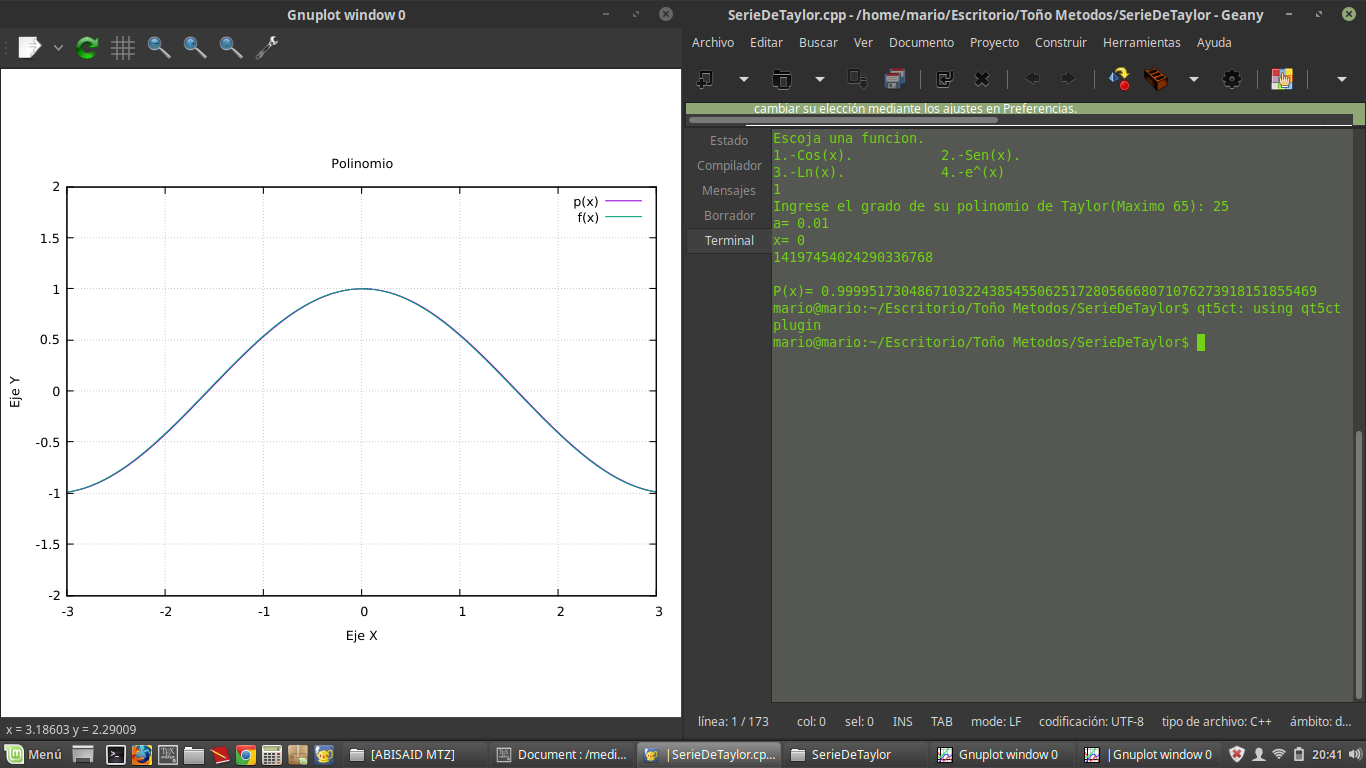
\includegraphics[scale=.125]{Taylor.png}
\caption{Programa con la condicion establecida}
\end{figure}
Observando la figura 1 se puede determinar el como la aproximacion estimada es correcta debido a que la aproximacion generada sobre esta debe de obtenerse $\cos x$ = 0.99995


\end{multicols}

\end{document}